\documentclass[conference,a4paper]{IEEEtran}

\usepackage[table,xcdraw]{xcolor}
% Escritura mejorada de fórmulas matemáticas
\usepackage{amsmath}
% Inserción de gráficos
\usepackage{graphicx}
\graphicspath{ {images/} }
% Escritura de pseudocódigo
\usepackage[kw]{pseudo}
\usepackage{algorithm}
\usepackage[noend]{algpseudocode}
% Escritura mejorada de tablas
\usepackage{booktabs}
% Escritura mejorada de citas bibliográficas
\usepackage{cite}
% Hipervínculos
\usepackage{hyperref}
\hypersetup{
    colorlinks=true,
    linkcolor=blue,
    filecolor=magenta,      
    urlcolor=cyan,
}
\urlstyle{same}

% Macros traducidas
\def\contentsname{Índice general}
\def\listfigurename{Índice de figuras}
\def\listtablename{Índice de tablas}
\def\refname{Referencias}
\def\indexname{Índice alfabético}
\def\figurename{Fig.}
\def\tablename{TABLA}
\def\partname{Parte}
\def\appendixname{Apéndice}
\def\abstractname{Resumen}
% IEEE specific names
\def\IEEEkeywordsname{Palabras clave}
\def\IEEEproofname{Demostración}

%Título
\title{Clustering con Incertidumbre}

%Autores
\author
{
	\IEEEauthorblockN{Víctor Muñoz Ramírez}
	\IEEEauthorblockA
	{
		\textit{Dpto. Ciencias de la Computación e Inteligencia Artificial}\\
		\textit{Universidad de Sevilla}\\
		Sevilla, España\\
		vicmunram@us.es
	}
	\and	
	\IEEEauthorblockN{Enrique Reina Gutiérrez}
	\IEEEauthorblockA
	{
		\textit{Dpto. Ciencias de la Computación e Inteligencia Artificial}\\
		\textit{Universidad de Sevilla}\\
		Sevilla, España\\
		enrreigut@us.es
	}
}

\begin{document}
\maketitle

%Investigación Kike

% Resumen
\begin{abstract}
El objetivo principal del trabajo es tratar de dar un catálogo de las posibles configuraciones con el objetivo de resolver diferentes escenarios de clustering, además de buscar un patrón en el comportamiento del algoritmo propuesto, para poder optimizar los tiempos de ejecución.

Las conclusiones obtenidas son, por lo general, que el método de clustering haciendo uso del circuncentro como técnica para la agrupación de los puntos funciona de una forma más precisa y aborda más escenarios, aunque suele ser mucho más lento (se explica esta causa a lo largo del trabajo), por ende existen situaciones donde interesa más el baricentro debido a motivos de velocidad. En casos de clusters simples que no se solapen o no sean concentricos, el baricentro es la opción elegir mientras que cuando las cosas se ponen un poco complejas interesa el circuncentro.
\end{abstract}

\begin{IEEEkeywords}
clustering, cluster(s), sorting, baricentro, circuncentro, concéntrica
\end{IEEEkeywords}

\section{Introducción}

En la gran mayoría de ámbitos, siempre hemos encontrado de forma muy útil la clasificación de datos con varios objetivos en mente como puede ser visualizar estos y ver que características comparten entre si.

Sin embargo, existe un problema, el tiempo. Dado un determinado conjunto de datos el cual posee un tamaño extenso, el tiempo que se puede llegar a invertir intentando clasificarlos de forma manual puede ser absurdamente grande.

Aquí es donde entra la ventaja de los ordenadores, pero ¿cómo? ¿Qué beneficio supondrá un ordenador en estos casos? 

Es cuando entramos en la rama de Inteligencia Artificial: Machine Learning, dentro del campo de aprendizaje no supervisado, donde aparece la técnica conocida como Clustering. Esta consiste en agrupar un conjunto de objetos no “etiquetados” en subconjuntos de objetos llamados clusters. Esa agrupación se realiza bajo la premisa que son similares.

El objetivo por abordar es poder encontrar un patrón en el comportamiento del algoritmo propuesto, para poder optimizar los tiempos de ejecución y obtener a modo de catálogo que opciones nos interesan más dados ciertos escenarios.

Esto resultará en la realización del código propuesto para resolver el problema de agrupación de puntos que conformen una circunferencia junto a una batería de ejemplos con diferentes configuraciones las cuales explicaremos con el fin de dar a entender lo que sucede, por qué y cómo mejorarlo.

De esta forma, tendremos como conclusión un conjunto de decisiones empíricas para diferentes configuraciones y diferentes escenarios donde podremos ver que nos interesa realizar.

%Marco teórico
\clearpage
\section{Marco Teórico}

Para la realización de nuestro trabajo, investigamos respecto al funcionamiento de los diferentes algoritmos utilizados.

Según la  \hyperref[bib:georgeSeif]{Referencia 1}:

Empieza con una pequeña introducción respecto a lo que es Clustering en Machine Learning. Una técnica para poder separar un conjunto de puntos dados. Estos puntos deben de poseer algún tipo de característica común que nos permita poder identificar unos de otros y así poder agruparlos.

Habla de 5 técnicas de algoritmos de Clustering: K-Means, Mean-Shift, Density-Based Spatial con Ruido, Expectation-Maximization (EM) usando mezcla de modelos Gaussianos (GMM) y Aglomerative Hierarchical Clustering. Cada uno presenta sus ventajas y desventajas, que iré desarrollando a lo largo de los siguientes puntos:\\

\paragraph{\textbf{K-Means}}

Este es el algoritmo que es presentado en las transparencias de teoría. Según el artículo es uno de los métodos más fácil de implementar y de entender. Lo primordialmente destacable es que el input inicial es tuyo, es decir, debes primero observar los datos y tratar de identificar el posible número o cantidad de grupos(clústeres) que puedes identificar según las densidades de los puntos.

Este algoritmo consiste, en como ya se mencionó anteriormente, seleccionar tantos puntos considerados como centros de los clusters que consideramos que hay según la representación dimensional de los datos. El algoritmo es iterativo, es decir, con cada iteración los centros se van desplazando de forma que se sitúen en el centro de cada clúster. Esto se consigue midiendo la distancia de los puntos con cada centro para ver a cuáles corresponden.

La ventaja de este método es que un algoritmo que es considerado bastante rápido con una complejidad de $\mathcal{O}(n)$. Sin embargo, partes con la premisa de que debes seleccionar una serie de clúster. Esta decisión no siempre es trivial. Una alternativa es realizar aproximaciones como, en función de la cantidad de puntos, introducir x centros, aunque puede provocar resultados diferentes, por ende resultando en una falta de consistencia.

Otra posible optimización de este algoritmo es ahorrarnos el tener que situar los puntos manualmente y simplemente indicar cuantos queremos. Esto suele realizarse mediante la inicialización aleatoria de estos puntos, no obstante, volvemos a encontrarnos con el problema de la falta de consistencia.

La solución a esta falta de consistencia sería el uso de generaciones (\hyperref[bib:clustering]{Referencia 2}). Instanciamos varias veces los clusteres con posiciones aleatorias y nos quedamos con el que de todas las generaciones agrupe de mejor forma los puntos.

Por otro lado, la Referencia ofrece una alternativa a K-Means conocida como K-Medians. La principal diferencia es que a la hora de recomputar los centros nos basamos en la mediana y no en la media. Este método es menos sensitivo a valores atípicos sin embargo es más costoso de forma computacional ya que requiere \textit{sorting} para computar la mediana del vector de los datos.\\

\paragraph{\textbf{Mean-Shift}}

Este algoritmo es un algoritmo basado en un enventanado que trata de encontrar las áreas más densas de puntos con el fin de determinar el centro de los clusters de puntos dados. Este algoritmo es denominado como \textit{centroid-base algorithym}. La función de este algoritmo es encontrar el centro de los clusters formado por el conjunto de puntos dados en función de la densidad de estos.

Lo primero que se hacer es inicializar un punto de forma aleatoria en el espacio de puntos con un radio de búsqueda. La superficie cubierta por el círculo (ventana circular la cual se le conoce como\textit{kernel} o núcleo) se encarga de contar los puntos incluidos en este. El vector dirección en el que se mueve se hace en función del centro de masa, es decir, donde se vayan concentrando los puntos.

La forma en la que este algoritmo converge es que, en vez de inicializar una única ventana, se inicializan varias distribuidas de forma uniforme por el espacio de puntos. Vamos iterando hasta que las distancia entre el centro de las ventanas sean cubiertas por todas las otras ventanas.

La ventaja de este algoritmo respecto a K-Means es que no requerimos de indicar el número de centros que vamos a necesitar, sino que se detectan solos basados en la densidad de puntos, sin embargo, esta ventaja que presenta puede llegar a ser una desventaja. Este método es perfecto para encontrar el centro de los puntos que formen parte de clusters que estén separados y sean densos. En el escenario de que los cluster conformen figuras, tipo el perímetro de un círculo, el algoritmo puede que no agrupe los puntos en único conjunto, sino que haga una subdivisión de estos. Otra desventaja que presenta es que se deben escoger la longitud del radio resultando factor determinista que puede provocar diferentes resultados.\\

\paragraph{\textbf{Density-Based Spatial Clustering con ruidos (DBSCAN)}}

Este algoritmo también está basado en la agrupación de los puntos en función de su densidad. La gran diferencia que presenta respecto a Mean-Shift es que no trata de localizar el centro del conjunto de los puntos, si no que va generando la agrupación al vuelo.

El funcionamiento del algoritmo es muy simple. Sen encarga de ir recorriendo todos los puntos del conjunto de puntos y mira en un radio alrededor de este. Si se encuentra un punto dentro de este radio, se le asigna como parte del clúster. Los puntos que se leen se marcan como visitados. En el momento que ha acabado de "agrupar un conjunto de puntos" pasa al siguiente en la lista de puntos.

Este algoritmo presenta ventajas respecto a K-Means ya que como en Mean-Shift no es necesario indicar de antemano el número de agrupaciones que identificamos o vamos a querer, además de que a difrencia de Mean-Shift es capaz de identificar figuras. Sin embargo, también tiene su desventaja la cual es que requiere cierta distancia mínima entre los puntos para poder agrupar todo en la misma figura, ya que la distancia a la que miramos, conocida como Epsilon, varía en función de la densidad de puntos en esa zona.\\

\paragraph{\textbf{Esperanza - Maximización utilizando Modelo de Mezclas Gaussianas (GMM)}}

Según las  \hyperref[bib:EM-GMM1]{Referencia 4} y \hyperref[bib:EM-GMM2]{Referencia 5}:

Esperanza - Maximización es un algoritmo estadístico para encontrar los parámetros de un modelo cuando los datos tienen variables desconocidas. Estas variables reciben el nombre de variables latentes y se busca optimizarlas utilizando la información de la que disponemos. Consiste en dos pasos:
\begin{itemize}
	\item Paso E (Esperanza): Usando los datos disponibles estimamos las variables latentes.\\
	\item Paso M (Maximización): Basándose en los valores estimados actualizamos el resto de parámetros maximizando el modelo.
\end{itemize}

En este caso, el modelo será el Modelo de Mezclas Gaussianas, el cual asume que los datos de entrada se encuentran organizados siguiendo distribuciones gaussianas. De este modo, nuestros clusters pasarán a ser dichas distribuciones las cuales tendrán tres parámetros: la media, la covarianza y el número de puntos que pertenecen a cada una de ellas, del que podremos obtener la densidad de la distribución.

En la inicialización del algoritmo se elige el número de clusters K de forma manual y se definen de forma aleatoria el resto de parámetros para cada cluster. La inicialización de estos últimos no es tan esencial como en otros algoritmos ya que se optimiza con mucha rapidez.\\
En cada iteración realizaremos dos pasos:

\begin{itemize}
	\item Paso E: Para cada punto del conjunto de datos calcularemos la probabilidad de que este pertenezca a cada uno de los clusters. Esta probabilidad es directamente proporcional a la distancia del punto al centro de la distribución gaussiana; ya que al utilizar este tipo de distribución asumimos que la mayoría de puntos se encuentran cercanos al centro del cluster. Se utiliza la siguiente fórmula:
\begin{gather}
\gamma_{k}(x)=\frac{\pi_{k}\textit{N}(x|\mu_{k},\Sigma_{k})}{\sum_{j=1}^{K}\pi_{j}\textit{N}(x|\mu_{j},\Sigma_{j})}\\
\gamma_{k}(x) \text{ = probabilidad de que } x \text{ pertenezca al cluster j}\\
\pi \text{ = densidad del cluster }\\
\textit{N}\text{ = Distribucion normal multivariante}\\
\mu \text{ y } \Sigma \text{ = media y covarianza del cluster}\\
x \text{ = un punto del conjunto de datos}
\end{gather}
	\item Paso M: Una vez calculado el paso anterior recalculamos los parámetros de cada cluster de forma que maximicen las probabilidades de pertenencia de cada punto a su cluster.
\begin{gather}
\pi_{j}=\frac{\sum_{n=1}^{N}\gamma_{j}(x_{n})}{\text{N}} \\
\mu_{j}=\frac{\sum_{n=1}^{N}\gamma_{j}(x_{n})x_{n}}{\sum_{n=1}^{N}\gamma_{j}(x_{n})}\\
\Sigma_{j}=\frac{\sum_{n=1}^{N}\gamma_{j}(x_{n})(x_{n}-\mu_{j})(x_{n}-\mu_{j})^T}{\sum_{n=1}^{N}\gamma_{j}(x_{n})}\\
\text{N = Número total de puntos}
\end{gather}

\end{itemize}

Las iteraciones se seguiran realizando hasta que se converja, es decir, que los parámetros de las distribuciones no varien mucho con respecto a los de la iteración anterior.\\

Este algoritmo aunque parecido a K-Medias presenta una serie de ventajas. La primera es que gracias a que utiliza además de la media la covarianza los clusters no están limitados a ser circunferencias, sino que pueden tomar cualquier tipo de forma elíptica; lo cual permite que el clustering se pueda realizar de forma correcta en casos en los que para K-Medias sería imposible, por ejemplo, en clusters concéntricos o clusters cuya forma no es circular. Además de esto, al funcionar con probabilidades, los puntos no tienen porqué pertenecer a un único cluster, sino que pueden tener una probabilidad de pertenencia a cada uno.

%Estructura del proyecto

\clearpage
\section{Preliminares}

\subsection{Métodos Empleados}

Al fin y al cabo la investigación realizada nos ayudó mucho a la hora de entender como abordar este problema (aún teniendo un algoritmo propuesto), ya que como se indica en la subsubsección de la investigación, un artículo nos dió la idea de hacer uso de una implementación de algoritmo genético. La idea es realizar varias inicializaciones con centros de cluster aleatorios y quedarnos con el mejor resultado trás la iteración de todas las generaciones.

Por otro lado, la técnica empleada es la misma que se indica en la propuesta del proyecto la cual es \textit{Clustering con Incertidumbre}. Simplemente inicializamos unos centros siguiendo algún tipo de heuirística o aleatoriedad. Calculamos la pertenencia de esos puntos a cada centro y actualizamos el centro y radio en función de los puntos que se asignen por iteración. Iteramos hasta que se alcanza el criterio de parada el cual es la convergencia de los clusters.

\section{Metodología}

\subsection{Dominio del problema y generación de ejemplos}

En primer lugar, se implementaron aquellas clases relativas a los elementos del dominio del problema, \textit{Point} y \textit{Circunference}, que sirven para representar el conjunto de puntos de entrada y las resultantes circunferencias que agrupan a estos.

La primera solo almacena las coordenadas x e y de un punto, mientras que la segunda almacena el centro y radio de una circunferencia; además del conjunto de puntos usados para su representación gráfica. Ambas clases, durante el desarrollo del proyecto, fueron aumentando en tamaño al incluirse en ellas métodos necesarios para la implementación del algoritmo.

Tras la elaboración de estas clases, se decidió diseñar las necesarias para la generación de ejemplos y representación gráfica de estos mismos. El objetivo era poder comprobar la eficacia de las distintas partes del algoritmo a medida que se desarrollaba con una buena variedad de casos de prueba; pudiéndose encontrar los fallos que podrían haberse cometido y subsanarlos lo antes posible.

Estas clases son \textit{DataSet} y  \textit{Canvas}, que nos permiten, respectivamente, realizar la carga de datos de un ejemplo a partir de un archivo .csv y elaborar y representar estos. En cuanto al formato de los archivos .csv, este viene detallado en el archivo README.txt adjunto al código. En cuanto a la generación de ejemplos, se crearon métodos aleatorios para la creación de distribuciones de circunferencias, la eliminación de un porcentaje de puntos y la inserción de ruido desviando estos. Este desvío se hace adaptando el método \textit{numpy.random.normal} el cual proporciona valores aleatorios dentro de una distribución. Para la adaptación solo es necesario aportar la desviación que queremos en dicha distribución.

La generación de un nuevo ejemplo consiste en crear una distribución aleatoria, eliminar algunos puntos de ella y desviar los restantes para tener algo de ruido. El único problema de esta forma de actuar, es que si se queremos un ejemplo muy concreto, es necesario crearlo a mano o bien ejecutar el método hasta tener un caso similar al buscado. Como ya se ha mencionado, \textit{Canvas} nos permite también representar dichos ejemplos mostrándonos de forma conjunta los puntos y circunferencias del problema.

\begin{figure}[H]
\centering
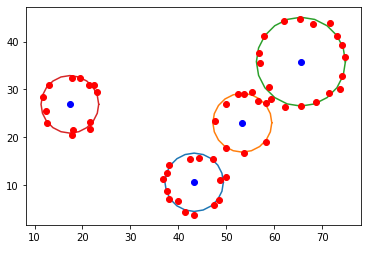
\includegraphics[scale=0.8]{EjemploGenerado}
\caption{Ejemplo generado de forma aleatoria, porcentaje de eliminación=30\%, escala del desvío=0.5}
\end{figure}

A continuación, se realizó la implementación de los objetivos específicos relativos al código siguiendo el orden en el que aparecían en el documento; ya que iban de menos a más en la elaboración del algoritmo final.

\subsection{Estructura de datos}

De esta manera, se diseñó para almacenar la información de cada iteración del algoritmo una estructura de datos basada en dos arrays: 
\begin{itemize}
	\item Clusters: Almacena objetos de la clase \textit{Circunference}, los cuales representan. El orden de estos en el array viene definido por como se inicializaron.
	\item Threshold: Almacena arrays con los grados de pertenencia de cada punto a cada cluster. El orden de estos viene definido por como estuvieran los puntos ordenados en el archivo .csv.
\end{itemize}

\subsection{Cálculo de circunferencias}

Tras esto, se elaboró un método para calcular centro y radio de una circunferencia a partir de un listado de puntos.

La primera versión de este método calculaba el centro como el baricentro del conjunto y el radio como la distancia media de este a todos los puntos. Este método, aunque muy eficiente incluso con ruido, fallaba cuando se le proporcionaba un arco en lugar de una circunferencia; ya que como el baricentro se sitúa en función de la densidad, el centro queda muy cerca del arco resultando en un radio menor al debido, y quedando los puntos de los extremos muy alejados de la circunferencia.

\begin{figure}[H]
\centering
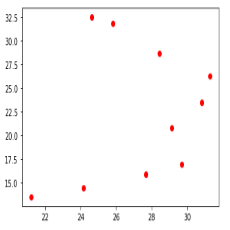
\includegraphics[scale=0.9]{ArcoBaricentro}
\caption{Ejemplo con los puntos en forma de arco}
\end{figure}

\begin{figure}[H]
\centering
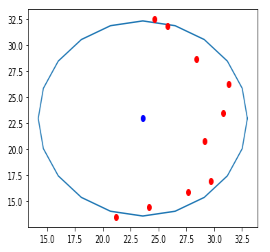
\includegraphics[scale=0.8]{ArcoBaricentroResultado}
\caption{Circunferencia calculada usando el baricentro}
\end{figure}

Por ello, se decidió implementar un segundo método que calculara el centro como el circuncentro del conjunto; ya que con la circunferencia circunscrita nos aseguramos que al menos pase por tres puntos de los proporcionados, y el radio como la distancia desde este a uno de esos puntos. Este se calcula como el punto de corte de las mediatrices de los segmentos que forman los puntos seleccionados, según \hyperref[bib:georgeSeif2]{Referencia 3}. El problema de esta forma de calcularlo es que los puntos elegidos hagan que las mediatrices no se corten y no haya solución, lo cual fue solventado haciendo que el cálculo se repitiera hasta que esta existiera.

\begin{figure}[H]
\centering
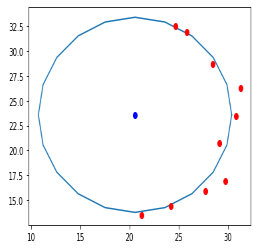
\includegraphics[scale=0.8]{ArcoCircuncentroResultado}
\caption{Circunferencia calculada usando el circuncentro}
\end{figure}

Como vemos, la selección de los puntos es muy importante y ha sido un elemento que se ha tratado de múltiples formas. El planteamiento inicial  consistía en tomar un punto aleatorio, buscar el más lejano a este y por último buscar uno a una distancia intermedia de ambos. Esta forma requería cierto coste computacional adiciona con respecto al baricentro;l ya que había que recorrer el listado de puntos más de una vez, pero reaccionaba bien incluso con arcos. Sin embargo, en situaciones con mucho ruido el resultado se desviaba. Se intentaron otras formas de seleccionar estos puntos, por ejemplo, siguiendo la estructura anterior pero siendo el último punto uno aleatorio también. Sin embargo, ninguna terminaba de funcionar; así que finalmente se optó porque todos fueran aleatorios ya que el resultado era muy similar y requería un coste computacional mucho menor.

Finalmente, se dejaron tanto el método que utiliza el baricentro como el que utiliza el circuncentro para poder comprobar con el algoritmo final como reaccionaba cada uno y cual era más eficiente.

\subsection{Cálculo de grados de pertenencia}

Después, se implementó el método correspondiente al cálculo de los grados de pertenencia.

Como primer paso se calculan todas las distancias del punto a los clusters, tras lo cual se realiza un sumatorio de todas ellas. A este se le restan las distancias por separado, para que los grados de pertenencia sean inversamente proporcionales a la distancia. Y para que dichos valores esten normalizados, se dividen los resultados de la operación anterior entre el sumatorio.

Cabe destacar que durante la experimentación con el algoritmo final, en ocasiones al intentar normalizar se producían divisiones por cero; lo cual fue solventado instanciando el sumatorio de los puntos con una cantidad despreciable.

Posteriormente, se diseñó una modificación de este método que calcula los grados de pertenencia para todos los puntos de un problema, devolviendo el array correspondiente a Threshold, ya mencionado antes. Para esto se llama al método anterior por cada uno de los puntos del problema.

\subsection{Implementación del esquema general}

Finalmente, se implementó la clase \textit{ClusteringSolver} en la cual encontramos el método \textit{learn}, el cual sigue el esquema general planteado con pequeñas modificaciones que comentaremos más adelante; pero primero vamos a centrarnos en lo que tienen en común ambas.

Para la inicialización, desde un inicio se decidió instanciar las circunferencias de forma aleatoria, concretamente, se toma como centro un punto aleatorio del listado y se le proporciona un radio también aleatorio. Además, se decidió permitir al usuario elegir si utilizar baricentro o circuncentro para recalcular las circunferencias. Aunque es cierto, que si el conjunto de puntos suministrado para un cluster es menor de tres, se utiliza el baricentro ya que el circuncentro necesita como minimo esa cantidad.

En cuanto al criterio de parada, primero se implementó con un número fijo de iteraciones ya que era más sencillo y permitía comprobar el comportamiento del algoritmo con facilidad; aunque finalmente se acabó implementando un criterio de parada basado en que los centros y radios de los clusters no variaran en una cantidad determinada por el usuario, correspondiente al parámetro \textit{precision}. Sin embargo, es necesario aportar un número máximo de iteraciones pues en el caso de utilizar el circuncentro para recalcular los clusters, al tomarse puntos aleatorios, los centros y radios pueden aumentar sustancialmente. Este problema no se produce al utilizar el baricentro.

Por último, para la presentación final de los datos, se creó la clase  \textit{Solution}; la cual utiliza la información contenida en un objeto \textit{ClusteringSolver} que ya ha realizado el método  \textit{learn}, es decir, ya ha obtenido el resultado del algoritmo. Esta clase nos permite eliminar puntos cuyo grado de pertenencia final sea menor al elegido por el usuario, además de representar los datos de forma gráfica mostrando las circunferencias junto con los puntos coloreados en función del cluster al que pertenecen. Si esta representación es de más de seis clusters,  los colores de puntos pertenecientes a distintas circunferencias se repetirán y no se podrá saber con certeza si la asignación es correcta; aunque aún será visible si las circunferencias se han definido correctamente.

Las modificaciones se realizaron una vez implementado todo. Realizando la experimentación se observó que la inicialización de los clusters al ser aleatoria condicionaba mucho el resultado final del algoritmo. De modo, que se decidió investigar sobre ello y se encontró que una técnica bastante utilizada era el lanzamiento del algoritmo con múltiples instancias haciendo uso de una heurística para obtener el mejor resultado de todas ellas. En nuestro caso, la heurística  considera un mejor resultado aquel en el que el sumatorio de las distancias de los puntos a los clusters es menor.

\subsection{Clases principales y sus métodos}

\underline{Clase \textit{Point}}:

Esta clase como su nombre indica representa un punto. Como constructor recibe las coordenadas del eje OX y el eje OY.

Como métodos adicionales en esta clase tenemos:

\begin{itemize}

	\item{\textbf{getFurthestPoints(points)	}: recibe como parámetro el conjunto de puntos y devuelve al más lejano de estos.}
	\item{\textbf{calculateDistanceToCluster(c)}: recibe como parámetro el cluster que queramos y con este llamamos al método auxiliar calculateDistanceToPoint(c) el cual recibe como parámetro el centro de ese cluster. El método deveulve la distancia al centro y simplemente le restamos el radio del cluster en valor absoluto.}
	\item{\textbf{calculateDistanceToCluster\_noAbs(c)}: recibe como parámetro el cluster que queramos y se comporta igual que el método anterior sin embargo en este método la distancia al cluster no está en valor absoluto.}
	\item{\textbf{calculateThreshold(clusters)}: recibe como parámetro el conjunto de clusters y devuelve el grado de pertenencia a estos. Para cada cluster calculamos la distancia y normalizamos de forma inversa el vector que resulta.}
	\item{\textbf{calculatePerpendicular(p)}: Recibe como parámetro otro punto y se devuelve el vector perpendicular al vector que resulta del punto al punto p.}
	\item{\textbf{calculateDistanceToPoint(p)}: recibe como parámetro un punto y se calcula la distancia euclídea a este.}
	\item{\textbf{equals(p)}: recibe como parámetro un punto y se comparan las componentes una a una para ver si son iguales.}
	\item{\textbf{print()}: se imprime las componentes del punto con el formato “(x,y)”.}

\end{itemize}

\underline{Clase \textit{Circunference}}:

Esta clase como su nombre indica, representa una circunferencia. Como constructor recibe un centro, un radio y un número de puntos (precisión a la hora de representar la circunferencia).

Como métodos adicionales en esta clase tenemos:

\begin{itemize}

	\item{\textbf{\_\_calculate()}: Método privado donde calculamos una representación de la circunferencia acorde con los parámetros que se pasan en el constructor.}
	\item{\textbf{update(centre, radius)}: Recibe como parámetro un centro y un radio que serán los valores a actualizar.}
	\item{\textbf{draw()}: Coge los valores calculados en el método calculate() y le damos una representación 2D. }
	\item{\textbf{drawPlot()}: Similar a draw() con la diferencia que se utiliza en otro contexto.}
	\item{\textbf{drawSubPlot(axs, it)}: Similar a draw() y recibe como parámetro unos eje (tipo de la librería matplotlib) y la iteración por la que va el algoritmo de aprendizaje.}
	\item{\textbf{calculateWithCircumcenter(points)}: Recibe como parámetro el conjunto de puntos de entre los cuales se escogen tres de forma aleatoria para realizar un circuncentro de estos y hacer una representación del cluster.}
	\item{\textbf{calculateWithBarycentre(list\_points)}: Recibe como parámetro la lista de puntos y se halla el baricentro haciendo una suma de las coordenadas del listado de puntos y dividiendo entre el total de puntos.  Para el radio hacemos una media de las distancias entre el baricentro y todos los puntos.}

\end{itemize}

\underline{Clase \textit{Clustering Solver}}:

Esta clase es la encargada de llevar a cabo el algoritmo de aprendizaje. Como constructor recibe una ruta a un fichero csv que contiene los puntos los cuales le queremos hacer clustering y la cantidad de custers con los que queremos que resuelva los puntos.

Como métodos adicionales tenemos:

\begin{itemize}

	\item{\textbf{initRandomClusters()}: Inicializa de forma aleatoria los clusters iniciales.}
	\item{\textbf{calculateThreshold()}: Calcula el grado de pertenencia de todos los puntos a cada cluster.}
	\item{\textbf{getClusterAssignment(threshold)}: Recibe como parámetro los grados de pertencia de cada punto a cada cluster. Con estos datos recorremos el vector de grados de pertenencia y a cada punto le asignamos un cluster según su pertenencia.}
	\item{\textbf{groupPointsByCluster(cluserAssignment)}: Recibe como parámetro el vector de tuplas (punto, cluster asigando) del método getClusterAssignment(threshold). Iteramos por todo el vector y vamos agrupando en función del cluster asignado. Devuelve un array de arrays con tantos grupos como clusteres con los puntos asignado a ese cluster.}
	\item{\textbf{calculateCluster(mode,points)}: Recibe como parámetro un modo que sirve para decidir si el cluster se va a formar mediante baricentro o circuncentro (mode puede ser ‘b’ o ‘c’) y los puntos asignado a ese cluster para formar la circunferencia que los agrupe.}
	\item{\textbf{learn(generations,precision,limit,mode)}: Recibe como parámetro el número de generaciones del algoritmo (cuantas veces se van a inicializar los clusters), la precisión que indica la mínima variación de una iteración a otra para que se considere que el algoritmos ha convergido, el límite que es el número de iteraciones máximas en el caso de que se encuentre en un bucle y el modo que al igual que en el método calculateCluster(mode,points) que define la técnica para definir la circunferencia que represente al cluster. En la subseccióon siguiente se mostrará el pseudocódigo de este algoritmo.

Este es el algorimto principal. Nos limitamos a instanciar un número de inicializaciones (generaciones) y vamos iterando hasta que converjan o se alcance el número de iteraciones máximas. Por cada generación nos guardamos la mejor iteración y de estas, comparamos la mejor para devolver la mejor asignación.}

\end{itemize}

\underline{Clase \textit{Solution}}:

Esta clase representa la solución final de haber realizado el algoritmo de asignación de clusters a los puntos, por ello el constructor recibe como parámetro la clase ClusteringSolver. Se limita a devolver el resultado aplicando un filtrado de detección de ruido, para que solo se devuelvan los puntos que realmente considera como suyos.

Como métodos adicionales tenemos:

\begin{itemize}

	\item{\textbf{eraseNoise(minThreshold)}: Recibe como parámetro el mínimo grado de pertenencia al cluster para que este se represente y no se considere como ruido. En caso de no cumplirse el grado de pertenencia mínimo ese punto es borrado.}

	\item{\textbf{drawSolution(minThreshold)}: Recibe como parámetro el mínimo grado de pertenencia ya que se llama al método auxiliar eraseNoise(minThreshold). Tras eliminar los puntos simplemente nos limitamos a dibujar los puntos con colores para que se pueda ver como se realizó la asignación de puntos a cada cluster.}

\end{itemize}

\subsection{Pseudocódigo}

\begin{figure}[H]
\begin{pseudo}*
\hd{\fn{learn}}(generations,precision,limit,mode) \\*
\multicolumn{2}{l}{\textbf{Entrada}: un entero  generations, un float precision,}\\*
\multicolumn{2}{l}{un entero limit y un boolean mode}\\*
\multicolumn{2}{l}{\textbf{Salida}: Ninguna (solo modifca valores ya existentes) } \\
mientras \( numGen \) \textnormal{es menor que generations} entonces \\+
inicializamos los clusters de forma aleatoria \\
mientras \( seguirIterando\) \textnormal{ $==$ 1 } entonces \\+
guardamos una copia de los clusters\\
calculamos la pertenencia\\
asignamos puntos a los clusters\\
agrupamos los puntos por cluster\\
por cada \( grupo de puntos en cluster \) \\+
calculamos centro y radio\\
si \textnormal{el radio es -1} entonces\\+
\( numGen \leftarrow \textnormal{numeGen - 1 }\) \\
asignamos la generation como sucia\\
break\\-
actualizamos los clusters\\
si \textnormal{la generation es sucia} entonces\\+
break\\-
por cada \textnormal{cluster guardado}\\+
\( centerCond \leftarrow \textnormal{difCentros $>$ precision} \)\\
\( radiusCond \leftarrow \textnormal{difRadius $>$ precision} \)\\
si \textnormal{centerCond or radiusCond} entonces\\+
\( dirtyIt \leftarrow 1 \) \\--
si \textnormal{dirtyIt $== 0$ or limitIt $==$ limit} entonces\\+
\(seguirIterando \leftarrow 0 \) \\-
\(limitIt \leftarrow limitIt + 1 \)\\-
si \textnormal{generation es la primera} entonces\\+
\(genClusters \leftarrow self.clusters\)\\
\(genAssignment \leftarrow clustersAssignment\)\\
por cada \textnormal{cluster en tempAssignment}\\+
\( genD \leftarrow \textnormal{genD + dist puntos al cluster}\) \\--
si no\\+
\(tempClusters \leftarrow self.clusters\)\\
\(tempAssignment \leftarrow clustersAssignment\)\\
por cada \textnormal{cluster en tempAssignment}\\+
\( dist \leftarrow \textnormal{dist + dist puntos al cluster}\) \\-
si \textnormal{dist $<genD$} entonces\\+
\( \textnormal{//Actualizamos los valores} \)\\
\(genClusters \leftarrow tempClusters\)\\
\(genAssignment \leftarrow tempAssignment\)\\
\( genD \leftarrow \textnormal{dist}\)\\-
\( numGen \leftarrow numGen + 1\)\\-
\(self.solCluster \leftarrow genClusters \) \\
\(self.solThres \leftarrow genAssignment \)
\end{pseudo}
\end{figure}

\subsection{Elementos descartados}

\textbf{Método para la selección de los tres puntos para realización del circuncentro:}

Originalmente habíamos diseñado un método que según cierta heurística era capaz de calcular el circuncentro de 3 puntos dados, sin embargo, siempre nos encontramos con el mismo problema de forma recursiva: no se escogían los puntos de la forma que queríamos.

Esto nos empujó a una solución un tanto radical que fue la selección de los puntos de forma aleatoria. Tal como se había planteado el algoritmo, esto no iban a suponer ningún problema ya que introdujimos generaciones, de forma que en alguna de ellas los puntos escogidos serían los ideales y efectivamente funcionaba.
Sin embargo, esto provocó un problema: Ciclos. Había un determinado momento en el que, por iteración al escogerse los puntos de forma aleatoria, los clusters variaban lo justo y necesario como para no converger.

Ante este problema teníamos tres soluciones: implementar un número máximo de iteraciones, subir el grado de precisión a valores poco precisos para considerar la convergencia o volver a intentar la selección de 3 puntos alejados entre sí de forma heurística.

Tras algunos intentos fallidos tratando de implementar alguna heurística para escoger siempre los mismos puntos para formar el cluster, decidimos mantener el algoritmo que escoge tres puntos aleatorios introduciendo un número máximo de iteraciones.

Presenta la ventaja de que el tiempo que invierte en generarse el cluster es siempre constante a expensas de que va a tardar en converger, alcanzando para la gran mayoría de casos las iteraciones máximas permitidas.

\textbf{Método iterativo:}

Tal como se indica en la propuesta del trabajo, existe la mejora de cambiar el código de iteración para que no se tenga que indicar un número de iteraciones con el fin de optimizar el algoritmo.

Este cambio se realiza simplemente introduciendo la precisión para la cual quieres que el algoritmo deje de iterar.

En nuestro caso, debido al problema explicado anteriormente solo se nos ve beneficiado en el caso en el que los clusters se formen con el total de los puntos (baricentros).

\subsection{Mejoras}

Como mejora, se implementó una interfaz gráfica dentro de Jupyter Notebook, que nos permite crear ejemplos aleatorios, eliminar de estos puntos, insertar ruido y guardarlos como fichero .csv en la ruta deseada; así como la resolución de estos indicando el número de instancias, clusters, precisión y máximo de iteraciones. Además, se aporta otra interfaz gráfica en la que se puede cargar un archivo .csv y resolverlo con los parámetros antes mencionados. Estos archivos siguen el formato indicado en el fichero README.txt.

Todo esto se proporciona al usuario a través de la clase \textit{ClusteringUI} y con los métodos \textit{createAndSolve} y \textit{loadAndSolve} que facilitan las funcionalidades anteriores. Esta interfaz deja al usuario de elegir los valores descritos anteriormente a través de sliders; así como insertarlos a mano.

\section{Resultados}

Para llevar a cabo la experimentación se crearon ejemplos para tratar tres escenarios bien diferenciados: circunferencias concéntricas, circunferencias solapadas y circunferencias separadas. Estos fueron probados con la cantidad correcta de clusters, uno más y uno menos. Además, de cada uno de estos ejemplos iniciales se obtuvieron otros cinco añadiéndoles ruido (ruido = 1.5 ó 0.5), eliminándoles puntos (porcentaje de eliminación = 0.6 ó 0.2) y aplicandoles ambos procedimientos (ruido = 0.4 y porcentaje de eliminación = 0.7). Estos fueron probados con la cantidad correcta de clusters únicamente.

El conjunto de ejemplos final ha sido probado con una precisión de 0.001, utilizando tanto el baricentro como el circuncentro, y aplicando las siguientes configuraciones: 1 generación y 10 iteraciones, 50 generaciones y 30 iteraciones; y 100 generaciones y 50 iteraciones. Para la primera configuración se realizaron tres ejecuciones del algoritmo para obtene la media del tiempo de ejecución y el porcentaje de fallos; mientras que para las otras no se consideró necesario ya que consisten en múltiples ejecuciones del algoritmo.

En las tablas de fallos 0 significa que no hubo fallo y 1 que sí.

\newpage
\subsection{Ejemplo 1: Circunferencias Concéntricas}

%Tablas
\begin{figure}[H]
\centering
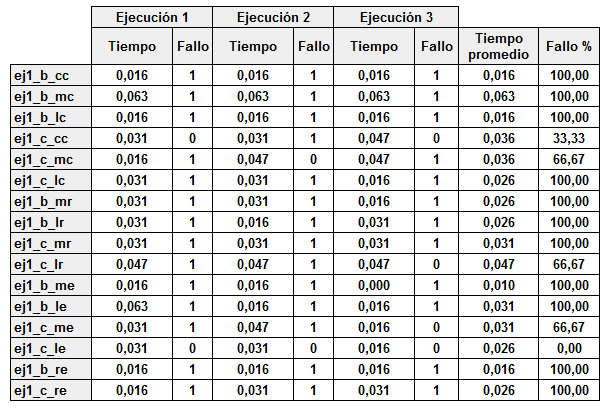
\includegraphics[scale=0.5]{Experimentacion/Ejemplo1/Ejemplo1Ejecuciones}
\caption{Ejemplo 1: Ejecuciones - Configuración 1}
\end{figure}

\begin{figure}[H]
\centering
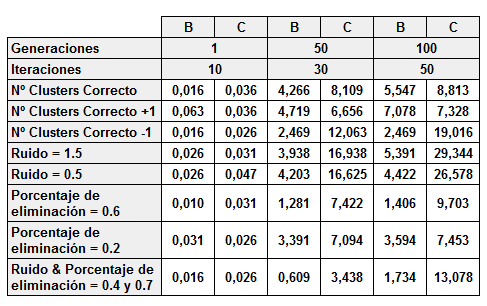
\includegraphics[scale=0.6]{Experimentacion/Ejemplo1/Ejemplo1Completo}
\caption{Ejemplo 1: Tiempos de todas la configuraciones}
\end{figure}

\begin{figure}[H]
\centering
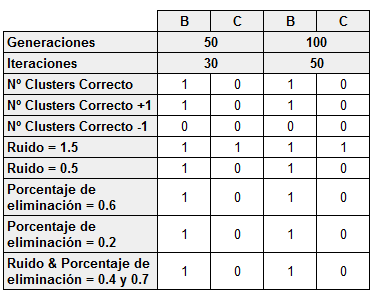
\includegraphics[scale=0.7]{Experimentacion/Ejemplo1/Ejemplo1Fallos}
\caption{Ejemplo 1: Fallos - Configuraciones 2 y 3}
\end{figure}

Se puede observar como con una sola generación el porcentaje de fallo es muy alto de forma general y que el circuncentro da mejores resultados que el baricentro. Además, destaca que al aumentar las generaciones e iteraciones el circuncentro mejora tanto que solo da fallo en presencia de mucho ruido; mientras que el baricentro solo mejora en el caso de realizarse el algoritmo con un número de cluster igual al correcto menos 1, pues agrupa las circunferencias concéntricas. También hay que destacar que el tiempo de ejecución del circuncentro es mucho mayor al del baricentro. Esto se repetirá en el resto de ejemplos.

%Ejemplo
\begin{figure}[H]
\centering
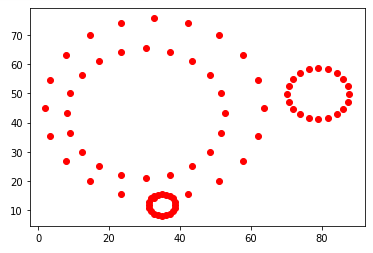
\includegraphics[scale=0.65]{Experimentacion/Ejemplo1/Ejemplo1}
\caption{Ejemplo 1: circunferencias concéntricas\\}
\end{figure}

%Capturas
\textbf{Pruebas con número de clusters:}\\

%Clusters-Baricentro
\begin{figure}[H]
\centering
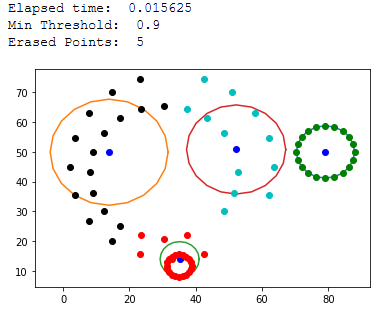
\includegraphics[scale=0.65]{Experimentacion/Ejemplo1/ej1_b_1_10_cc}
\caption{Ejemplo 1: Baricentro, 1 Generación y 10 Iteraciones,  Nº Clusters Correcto, Fallo\\}
\end{figure}

\begin{figure}[H]
\centering
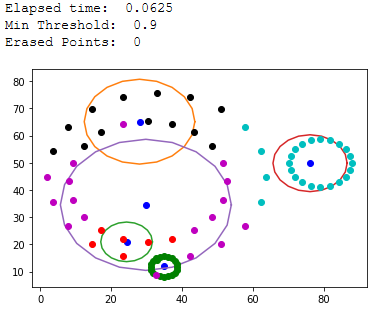
\includegraphics[scale=0.65]{Experimentacion/Ejemplo1/ej1_b_1_10_mc}
\caption{Ejemplo 1: Baricentro, 1 Generación y 10 Iteraciones,  Nº Clusters Correcto +1, Fallo\\}
\end{figure}

\begin{figure}[H]
\centering
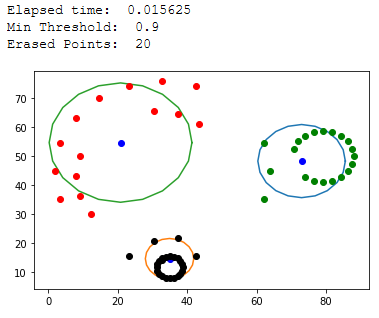
\includegraphics[scale=0.65]{Experimentacion/Ejemplo1/ej1_b_1_10_lc}
\caption{Ejemplo 1: Baricentro, 1 Generación y 10 Iteraciones,  Nº Clusters Correcto -1, Fallo\\}
\end{figure}

%Clusters-Circuncentro
\begin{figure}[H]
\centering
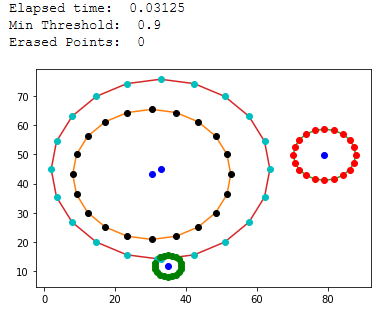
\includegraphics[scale=0.65]{Experimentacion/Ejemplo1/ej1_c_1_10_cc}
\caption{Ejemplo 1: Circuncentro, 1 Generación y 10 Iteraciones,  Nº Clusters Correcto, Acierto\\}
\end{figure}

\begin{figure}[H]
\centering
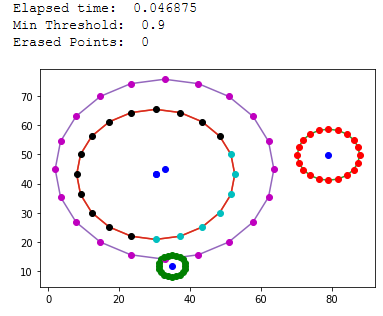
\includegraphics[scale=0.65]{Experimentacion/Ejemplo1/ej1_c_1_10_mc_correct}
\caption{Ejemplo 1: Circuncentro, 1 Generación y 10 Iteraciones,  Nº Clusters Correcto +1, Acierto\\}
\end{figure}

\begin{figure}[H]
\centering
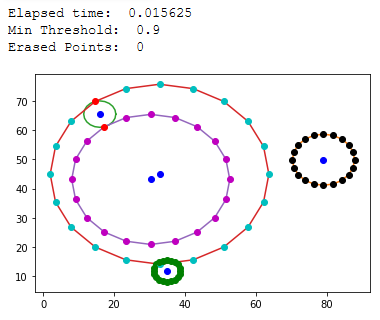
\includegraphics[scale=0.65]{Experimentacion/Ejemplo1/ej1_c_1_10_mc_wrong}
\caption{Ejemplo 1: Circuncentro, 1 Generación y 10 Iteraciones,  Nº Clusters Correcto +1, Fallo\\}
\end{figure}

\begin{figure}[H]
\centering
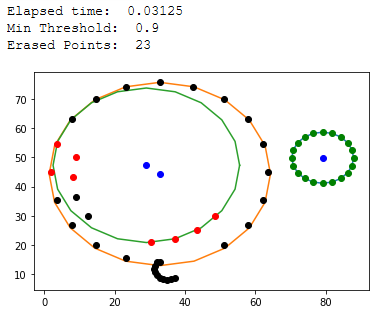
\includegraphics[scale=0.65]{Experimentacion/Ejemplo1/ej1_c_1_10_lc}
\caption{Ejemplo 1: Circuncentro, 1 Generación y 10 Iteraciones,  Nº Clusters Correcto -1, Fallo\\}
\end{figure}

\textbf{Pruebas con ruido:}\\

%Ruido-Baricentro
\begin{figure}[H]
\centering
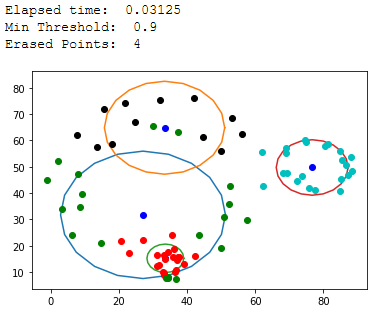
\includegraphics[scale=0.65]{Experimentacion/Ejemplo1/ej1_b_1_10_mr}
\caption{Ejemplo 1: Baricentro, 1 Generación y 10 Iteraciones,  Nº Clusters Correcto, Ruido = 1.5, Fallo\\}
\end{figure}

\begin{figure}[H]
\centering
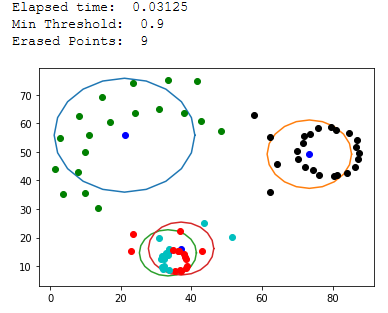
\includegraphics[scale=0.65]{Experimentacion/Ejemplo1/ej1_b_1_10_lr}
\caption{Ejemplo 1: Baricentro, 1 Generación y 10 Iteraciones,  Nº Clusters Correcto, Ruido = 0.5, Fallo\\}
\end{figure}

%Ruido-Circuncentro
\begin{figure}[H]
\centering
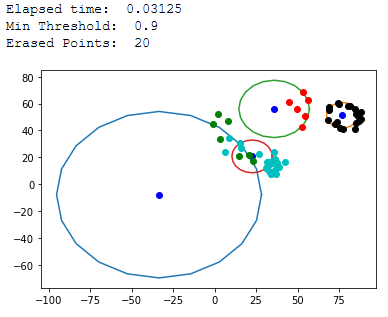
\includegraphics[scale=0.65]{Experimentacion/Ejemplo1/ej1_c_1_10_mr}
\caption{Ejemplo 1: Circuncentro, 1 Generación y 10 Iteraciones,  Nº Clusters Correcto, Ruido = 1.5, Fallo\\}
\end{figure}

\begin{figure}[H]
\centering
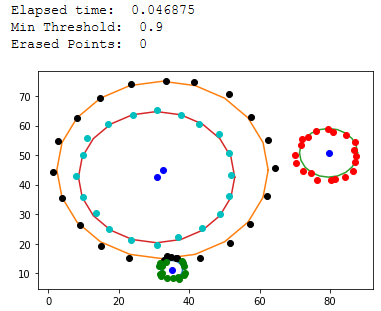
\includegraphics[scale=0.65]{Experimentacion/Ejemplo1/ej1_c_1_10_lr_correct}
\caption{Ejemplo 1: Circuncentro, 1 Generación y 10 Iteraciones,  Nº Clusters Correcto, Ruido = 0.5, Acierto\\}
\end{figure}

\begin{figure}[H]
\centering
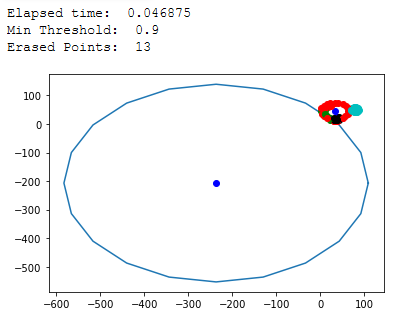
\includegraphics[scale=0.65]{Experimentacion/Ejemplo1/ej1_c_1_10_lr_wrong}
\caption{Ejemplo 1: Circuncentro, 1 Generación y 10 Iteraciones,  Nº Clusters Correcto, Ruido = 0.5, Fallo\\}
\end{figure}

\textbf{Pruebas con eliminación:}\\

%Eliminación-Baricentro
\begin{figure}[H]
\centering
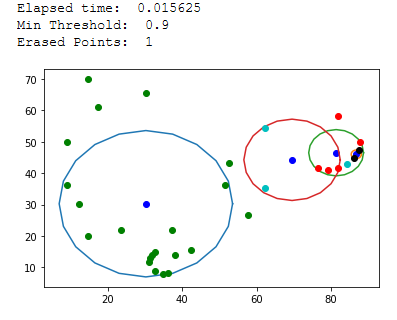
\includegraphics[scale=0.65]{Experimentacion/Ejemplo1/ej1_b_1_10_me}
\caption{Ejemplo 1: Baricentro, 1 Generación y 10 Iteraciones,  Nº Clusters Correcto, Porcentaje de eliminación = 0.6, Fallo\\}
\end{figure}

\begin{figure}[H]
\centering
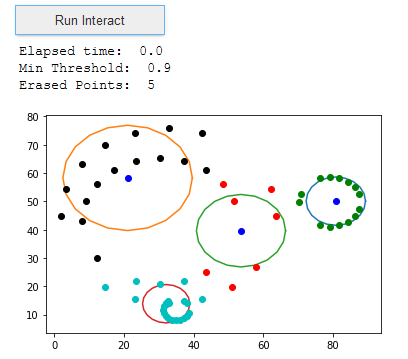
\includegraphics[scale=0.65]{Experimentacion/Ejemplo1/ej1_b_1_10_le}
\caption{Ejemplo 1: Baricentro, 1 Generación y 10 Iteraciones,  Nº Clusters Correcto, Porcentaje de eliminación = 0.2, Fallo\\}
\end{figure}

%Eliminación-Circuncentro
\begin{figure}[H]
\centering
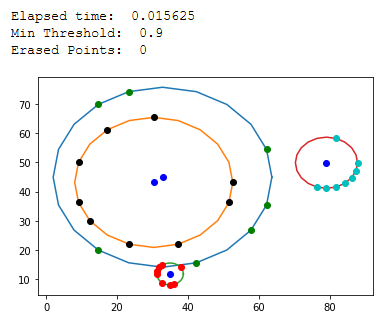
\includegraphics[scale=0.65]{Experimentacion/Ejemplo1/ej1_c_1_10_me_correct}
\caption{Ejemplo 1: Circuncentro, 1 Generación y 10 Iteraciones,  Nº Clusters Correcto, Porcentaje de eliminación = 0.6, Acierto\\}
\end{figure}

\begin{figure}[H]
\centering
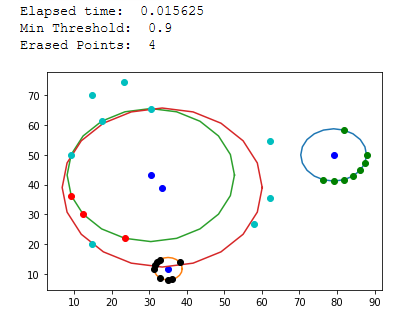
\includegraphics[scale=0.65]{Experimentacion/Ejemplo1/ej1_c_1_10_me_wrong}
\caption{Ejemplo 1: Circuncentro, 1 Generación y 10 Iteraciones,  Nº Clusters Correcto, Porcentaje de eliminación = 0.6, Fallo\\}
\end{figure}

\begin{figure}[H]
\centering
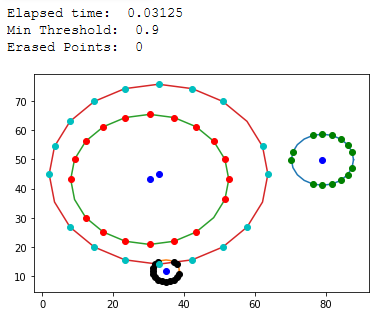
\includegraphics[scale=0.65]{Experimentacion/Ejemplo1/ej1_c_1_10_le}
\caption{Ejemplo 1: Circuncentro, 1 Generación y 10 Iteraciones,  Nº Clusters Correcto, Porcentaje de eliminación = 0.2, Acierto\\}
\end{figure}

\newpage
\textbf{Pruebas con eliminación y ruido:}\\

%Ruido-Eliminación
\begin{figure}[H]
\centering
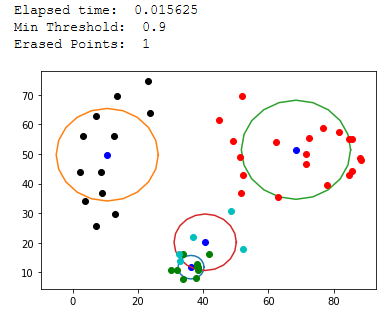
\includegraphics[scale=0.65]{Experimentacion/Ejemplo1/ej1_b_1_10_re}
\caption{Ejemplo 1: Baricentro, 1 Generación y 10 Iteraciones,  Nº Clusters Correcto, Ruido = 0.7, Porcentaje de eliminación = 0.4, Fallo\\}
\end{figure}

\begin{figure}[H]
\centering
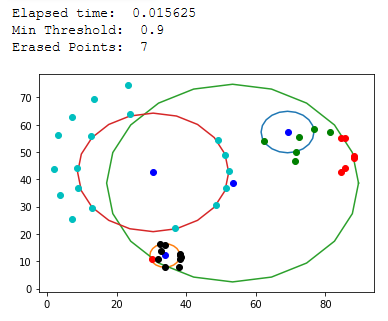
\includegraphics[scale=0.65]{Experimentacion/Ejemplo1/ej1_c_1_10_re_wrong}
\caption{Ejemplo 1: Circuncentro, 1 Generación y 10 Iteraciones,  Nº Clusters Correcto, Ruido = 0.7, Porcentaje de eliminación = 0.4, Fallo\\}
\end{figure}

\newpage
\subsection{Ejemplo 2: Circunferencias Solapadas}

%Tablas
\begin{figure}[H]
\centering
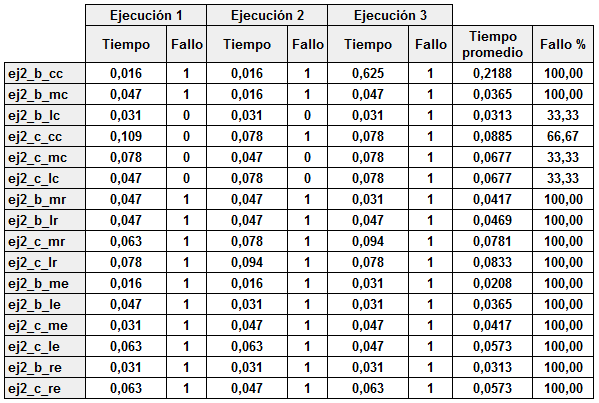
\includegraphics[scale=0.5]{Experimentacion/Ejemplo2/Ejemplo2Ejecuciones}
\caption{Ejemplo 2: Ejecuciones - Configuración 1\\}
\end{figure}

\begin{figure}[H]
\centering
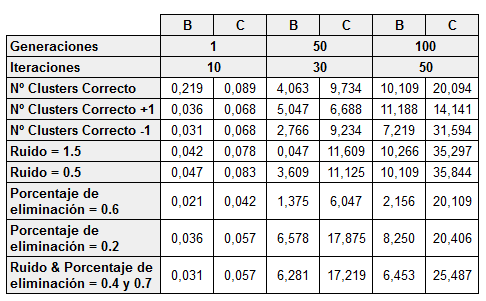
\includegraphics[scale=0.6]{Experimentacion/Ejemplo2/Ejemplo2Completo}
\caption{Ejemplo 2: Tiempos de todas la configuraciones\\}
\end{figure}

\begin{figure}[H]
\centering
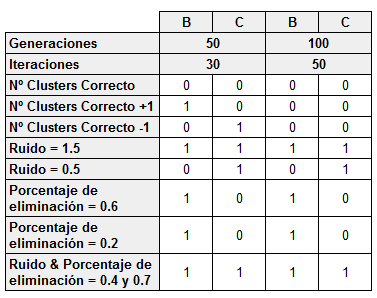
\includegraphics[scale=0.7]{Experimentacion/Ejemplo2/Ejemplo2Fallos}
\caption{Ejemplo 2: Fallos - Configuraciones 2 y 3\\}
\end{figure}

De nuevo el porcentaje de fallo es muy alto para una sola generación y se observa una mejoría destacable aumentando las generaciones e iteraciones. Además, el circuncentro muestra otra vez un mayor nivel de mejora salvo en presencia de mucho ruido; donde el baricentro responde mejor. Sin embargo, ambos muestran buenos resultados en presencia de ruido pero con un menor número de solapamientos, esto se puede observar con un ejemplo adicional con menor solapamiento añadido al final de esta sección.

%Ejemplo
\begin{figure}[H]
\centering
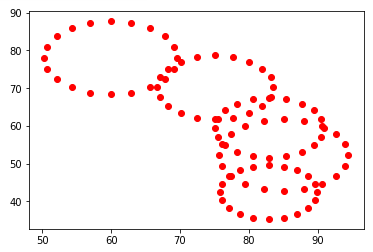
\includegraphics[scale=0.65]{Experimentacion/Ejemplo2/Ejemplo2}
\caption{Ejemplo 2: circunferencias solapadas}
\end{figure}

%Capturas

\textbf{Pruebas con número de clusters:}\\

%Clusters-Baricentro
\begin{figure}[H]
\centering
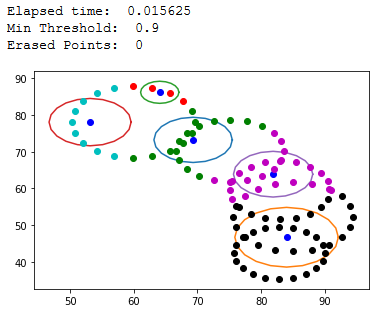
\includegraphics[scale=0.65]{Experimentacion/Ejemplo2/ej2_b_1_10_cc_wrong}
\caption{Ejemplo 2: Baricentro, 1 Generación y 10 Iteraciones,  Nº Clusters Correcto, Fallo\\}
\end{figure}

\begin{figure}[H]
\centering
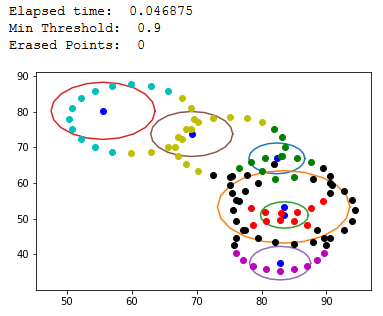
\includegraphics[scale=0.65]{Experimentacion/Ejemplo2/ej2_b_1_10_mc_wrong}
\caption{Ejemplo 2: Baricentro, 1 Generación y 10 Iteraciones,  Nº Clusters Correcto +1, Fallo\\}
\end{figure}

\begin{figure}[H]
\centering
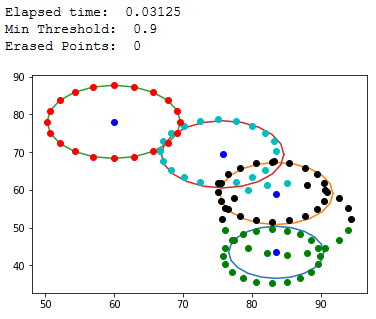
\includegraphics[scale=0.65]{Experimentacion/Ejemplo2/ej2_b_1_10_lc_correct}
\caption{Ejemplo 2: Baricentro, 1 Generación y 10 Iteraciones,  Nº Clusters Correcto -1, Acierto\\}
\end{figure}

\begin{figure}[H]
\centering
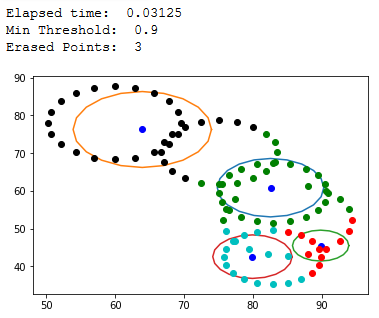
\includegraphics[scale=0.65]{Experimentacion/Ejemplo2/ej2_b_1_10_lc_wrong}
\caption{Ejemplo 2: Baricentro, 1 Generación y 10 Iteraciones,  Nº Clusters Correcto -1, Fallo\\}
\end{figure}

%Clusters-Circuncentro
\begin{figure}[H]
\centering
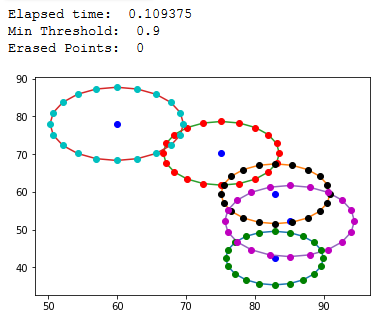
\includegraphics[scale=0.65]{Experimentacion/Ejemplo2/ej2_c_1_10_cc_correct}
\caption{Ejemplo 2: Circuncentro, 1 Generación y 10 Iteraciones,  Nº Clusters Correcto, Acierto\\}
\end{figure}

\begin{figure}[H]
\centering
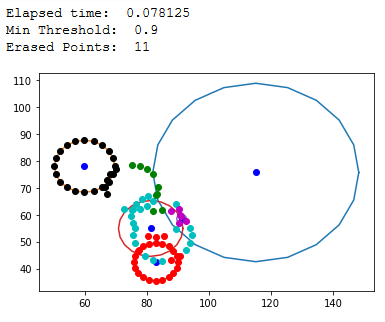
\includegraphics[scale=0.65]{Experimentacion/Ejemplo2/ej2_c_1_10_cc_wrong}
\caption{Ejemplo 2: Circuncentro, 1 Generación y 10 Iteraciones,  Nº Clusters Correcto, Fallo\\}
\end{figure}

\begin{figure}[H]
\centering
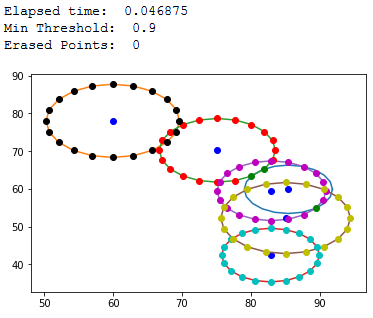
\includegraphics[scale=0.65]{Experimentacion/Ejemplo2/ej2_c_1_10_mc_correct}
\caption{Ejemplo 2: Circuncentro, 1 Generación y 10 Iteraciones,  Nº Clusters Correcto +1, Acierto\\}
\end{figure}

\begin{figure}[H]
\centering
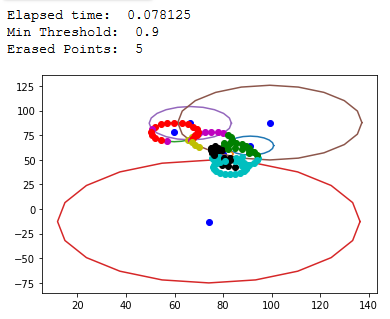
\includegraphics[scale=0.65]{Experimentacion/Ejemplo2/ej2_c_1_10_mc_wrong}
\caption{Ejemplo 2: Circuncentro, 1 Generación y 10 Iteraciones,  Nº Clusters Correcto +1, Fallo\\}
\end{figure}

\begin{figure}[H]
\centering
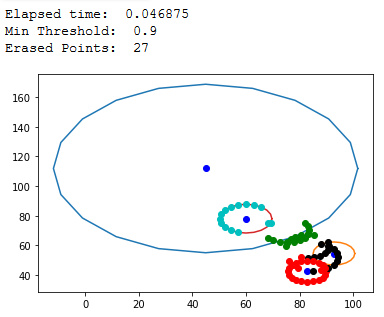
\includegraphics[scale=0.65]{Experimentacion/Ejemplo2/ej2_c_1_10_lc_wrong}
\caption{Ejemplo 2: Circuncentro, 1 Generación y 10 Iteraciones,  Nº Clusters Correcto -1, Fallo\\}
\end{figure}

\textbf{Pruebas con ruido:}\\

%Ruido-Baricentro
\begin{figure}[H]
\centering
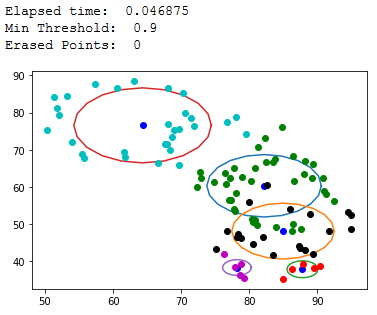
\includegraphics[scale=0.65]{Experimentacion/Ejemplo2/ej2_b_1_10_mr_wrong}
\caption{Ejemplo 2: Baricentro, 1 Generación y 10 Iteraciones,  Nº Clusters Correcto, Ruido = 1.5, Fallo\\}
\end{figure}

\begin{figure}[H]
\centering
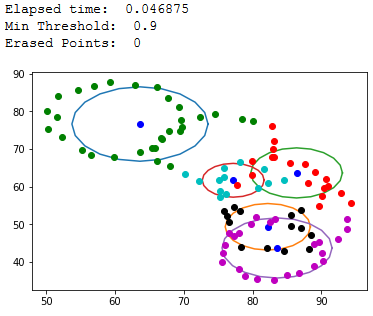
\includegraphics[scale=0.65]{Experimentacion/Ejemplo2/ej2_b_1_10_lr_wrong}
\caption{Ejemplo 2: Baricentro, 1 Generación y 10 Iteraciones,  Nº Clusters Correcto, Ruido = 0.5, Fallo\\}
\end{figure}

%Ruido-Circuncentro
\begin{figure}[H]
\centering
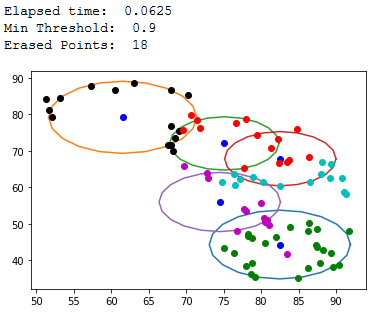
\includegraphics[scale=0.65]{Experimentacion/Ejemplo2/ej2_c_1_10_mr_wrong}
\caption{Ejemplo 2: Circuncentro, 1 Generación y 10 Iteraciones,  Nº Clusters Correcto, Ruido = 1.5, Fallo\\}
\end{figure}

\begin{figure}[H]
\centering
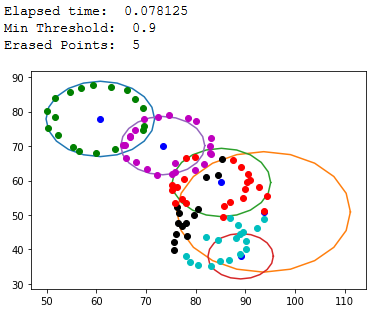
\includegraphics[scale=0.65]{Experimentacion/Ejemplo2/ej2_c_1_10_lr_wrong}
\caption{Ejemplo 2: Circuncentro, 1 Generación y 10 Iteraciones,  Nº Clusters Correcto, Ruido = 0.5, Fallo\\\\\\}
\end{figure}

\textbf{Pruebas con eliminación:}\\

%Eliminación-Baricentro
\begin{figure}[H]
\centering
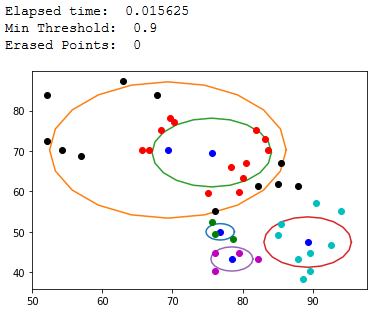
\includegraphics[scale=0.65]{Experimentacion/Ejemplo2/ej2_b_1_10_me_wrong}
\caption{Ejemplo 2: Baricentro, 1 Generación y 10 Iteraciones,  Nº Clusters Correcto, Porcentaje de eliminación = 0.6, Fallo\\}
\end{figure}

\begin{figure}[H]
\centering
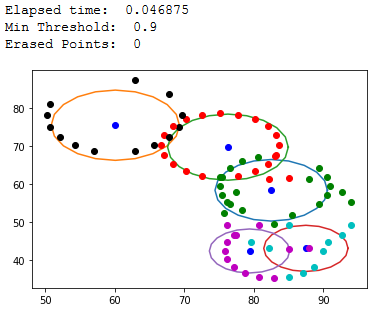
\includegraphics[scale=0.65]{Experimentacion/Ejemplo2/ej2_b_1_10_le_wrong}
\caption{Ejemplo 2: Baricentro, 1 Generación y 10 Iteraciones,  Nº Clusters Correcto, Porcentaje de eliminación = 0.2, Fallo\\}
\end{figure}

%Eliminación-Circuncentro
\begin{figure}[H]
\centering
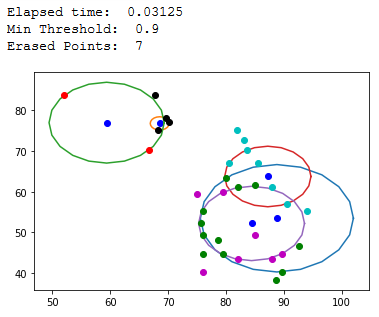
\includegraphics[scale=0.65]{Experimentacion/Ejemplo2/ej2_c_1_10_me_wrong}
\caption{Ejemplo 2: Circuncentro, 1 Generación y 10 Iteraciones,  Nº Clusters Correcto, Porcentaje de eliminación = 0.6, Fallo\\}
\end{figure}

\begin{figure}[H]
\centering
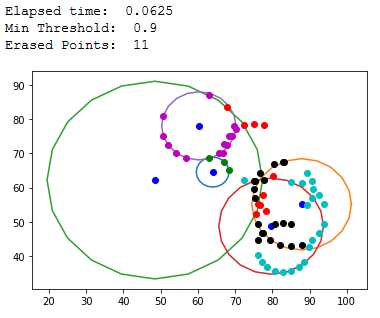
\includegraphics[scale=0.65]{Experimentacion/Ejemplo2/ej2_c_1_10_le_wrong}
\caption{Ejemplo 2: Circuncentro, 1 Generación y 10 Iteraciones,  Nº Clusters Correcto, Porcentaje de eliminación = 0.2, Fallo\\}
\end{figure}

\newpage
\textbf{Pruebas con eliminación y ruido:}\\

%Ruido-Eliminación
\begin{figure}[H]
\centering
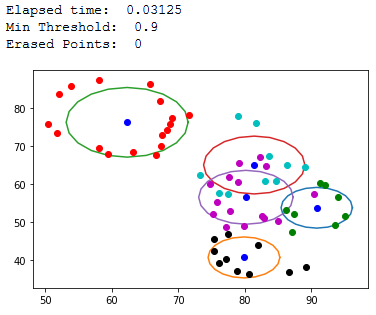
\includegraphics[scale=0.65]{Experimentacion/Ejemplo2/ej2_b_1_10_re_wrong}
\caption{Ejemplo 2: Baricentro, 1 Generación y 10 Iteraciones,  Nº Clusters Correcto, Ruido = 0.7, Porcentaje de eliminación = 0.4, Fallo\\}
\end{figure}

\begin{figure}[H]
\centering
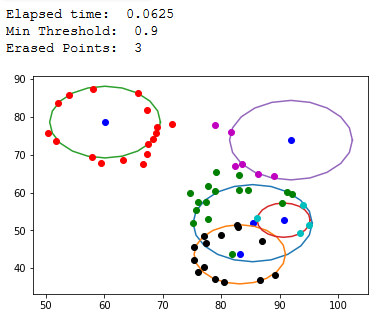
\includegraphics[scale=0.65]{Experimentacion/Ejemplo2/ej2_c_1_10_re_wrong}
\caption{Ejemplo 2: Circuncentro, 1 Generación y 10 Iteraciones,  Nº Clusters Correcto, Ruido = 0.7, Porcentaje de eliminación = 0.4, Fallo\\}
\end{figure}

\textbf{Ejemplo con menor solapamiento, Ruido = 1.5:}\\

%EjemploMenorSolapamiento
\begin{figure}[H]
\centering
\includegraphics[scale=0.8]{Experimentacion/EjemploMenorSolapamiento/EjemploMenorSolapamientoMaxRuido}
\caption{Ejemplo con menor solapamiento, Ruido = 1.5}
\end{figure}

\begin{figure}[H]
\centering
\includegraphics[scale=0.65]{Experimentacion/EjemploMenorSolapamiento/ejms_b_100_50_mr_correct}
\caption{Ejemplo con menor solapamiento: Baricentro, 100 Generaciones y 50 Iteraciones,  Nº Clusters Correcto, Ruido = 1.5, Acierto\\}
\end{figure}

\begin{figure}[H]
\centering
\includegraphics[scale=0.65]{Experimentacion/EjemploMenorSolapamiento/ejms_c_100_50_mr_correct}
\caption{Ejemplo con menor solapamiento: Circuncentro, 100 Generaciones y 50 Iteraciones,  Nº Clusters Correcto, Ruido = 1.5, Acierto\\}
\end{figure}

\textbf{Ejemplo con menor solapamiento, Ruido = 0.7, Porcentaje de Eliminación = 0.4:}\\

\begin{figure}[H]
\centering
\includegraphics[scale=0.8]{Experimentacion/EjemploMenorSolapamiento/EjemploMenorSolapamientoElimRuido}
\caption{Ejemplo con menor solapamiento, porcentaje de eliminación = 0.4, ruido = 0.7}
\end{figure}

\begin{figure}[H]
\centering
\includegraphics[scale=0.65]{Experimentacion/EjemploMenorSolapamiento/ejms_b_100_50_re_correct}
\caption{Ejemplo con menor solapamiento: Baricentro, 100 Generaciones y 50 Iteraciones,  Nº Clusters Correcto, Ruido = 0.7, Porcentaje de Eliminación = 0.4, Acierto\\}
\end{figure}

\begin{figure}[H]
\centering
\includegraphics[scale=0.65]{Experimentacion/EjemploMenorSolapamiento/ejms_c_100_50_re_correct}
\caption{Ejemplo con menor solapamiento: Circuncentro, 100 Generaciones y 50 Iteraciones,  Nº Clusters Correcto, Ruido = 0.7, Porcentaje de Eliminación = 0.4, Acierto\\}
\end{figure}

\newpage
\subsection{Ejemplo 3: Circunferencias Separadas}

%Tablas
\begin{figure}[H]
\centering
\includegraphics[scale=0.5]{Experimentacion/Ejemplo3/Ejemplo3Ejecuciones}
\caption{Ejemplo 3: Ejecuciones - Configuración 1\\}
\end{figure}

\begin{figure}[H]
\centering
\includegraphics[scale=0.6]{Experimentacion/Ejemplo3/Ejemplo3Completo}
\caption{Ejemplo 3: Tiempos de todas la configuraciones\\}
\end{figure}

\begin{figure}[H]
\centering
\includegraphics[scale=0.7]{Experimentacion/Ejemplo3/Ejemplo3Fallos}
\caption{Ejemplo 3: Fallos - Configuraciones 2 y 3\\}
\end{figure}

En este ejemplo el porcentaje de fallo con una sola generación es mucho menor al de los anteriores, observándose que los fallos se concentran en las pruebas con eliminación principalmente. Además, se puede observar que el aumento de generaciones e iteraciones produce una mejora tan notable que ya con la segunda configuración no se presenta ningún fallo.

%Ejemplo
\begin{figure}[H]
\centering
\includegraphics[scale=0.65]{Experimentacion/Ejemplo3/Ejemplo3}
\caption{Ejemplo 3: circunferencias separadas}
\end{figure}

%Capturas

\textbf{Pruebas con número de clusters:}\\

%Clusters-Baricentro
\begin{figure}[H]
\centering
\includegraphics[scale=0.65]{Experimentacion/Ejemplo3/ej3_b_1_10_cc_correct}
\caption{Ejemplo 3: Baricentro, 1 Generación y 10 Iteraciones,  Nº Clusters Correcto, Acierto\\}
\end{figure}

\begin{figure}[H]
\centering
\includegraphics[scale=0.65]{Experimentacion/Ejemplo3/ej3_b_1_10_cc_wrong}
\caption{Ejemplo 3: Baricentro, 1 Generación y 10 Iteraciones,  Nº Clusters Correcto, Fallo\\}
\end{figure}

\begin{figure}[H]
\centering
\includegraphics[scale=0.65]{Experimentacion/Ejemplo3/ej3_b_1_10_mc_correct}
\caption{Ejemplo 3: Baricentro, 1 Generación y 10 Iteraciones,  Nº Clusters Correcto +1, Acierto\\}
\end{figure}

\begin{figure}[H]
\centering
\includegraphics[scale=0.65]{Experimentacion/Ejemplo3/ej3_b_1_10_mc_correct2}
\caption{Ejemplo 3: Baricentro, 1 Generación y 10 Iteraciones,  Nº Clusters Correcto +1, Acierto\\}
\end{figure}

\begin{figure}[H]
\centering
\includegraphics[scale=0.65]{Experimentacion/Ejemplo3/ej3_b_1_10_mc_wrong}
\caption{Ejemplo 3: Baricentro, 1 Generación y 10 Iteraciones,  Nº Clusters Correcto +1, Fallo\\}
\end{figure}

\begin{figure}[H]
\centering
\includegraphics[scale=0.65]{Experimentacion/Ejemplo3/ej3_b_1_10_lc_correct}
\caption{Ejemplo 3: Baricentro, 1 Generación y 10 Iteraciones,  Nº Clusters Correcto -1, Acierto\\}
\end{figure}

\begin{figure}[H]
\centering
\includegraphics[scale=0.65]{Experimentacion/Ejemplo3/ej3_b_1_10_lc_wrong}
\caption{Ejemplo 3: Baricentro, 1 Generación y 10 Iteraciones,  Nº Clusters Correcto -1, Fallo\\}
\end{figure}

%Clusters-Circuncentro
\begin{figure}[H]
\centering
\includegraphics[scale=0.65]{Experimentacion/Ejemplo3/ej3_c_1_10_cc_correct}
\caption{Ejemplo 3: Circuncentro, 1 Generación y 10 Iteraciones,  Nº Clusters Correcto, Acierto\\}
\end{figure}

\begin{figure}[H]
\centering
\includegraphics[scale=0.65]{Experimentacion/Ejemplo3/ej3_c_1_10_cc_wrong}
\caption{Ejemplo 3: Circuncentro, 1 Generación y 10 Iteraciones,  Nº Clusters Correcto, Fallo\\}
\end{figure}

\begin{figure}[H]
\centering
\includegraphics[scale=0.65]{Experimentacion/Ejemplo3/ej3_c_1_10_mc_correct}
\caption{Ejemplo 3: Circuncentro, 1 Generación y 10 Iteraciones,  Nº Clusters Correcto +1, Acierto\\}
\end{figure}

\begin{figure}[H]
\centering
\includegraphics[scale=0.65]{Experimentacion/Ejemplo3/ej3_c_1_10_mc_correct2}
\caption{Ejemplo 3: Circuncentro, 1 Generación y 10 Iteraciones,  Nº Clusters Correcto +1, Acierto\\}
\end{figure}

\begin{figure}[H]
\centering
\includegraphics[scale=0.65]{Experimentacion/Ejemplo3/ej3_c_1_10_lc}
\caption{Ejemplo 3: Circuncentro, 1 Generación y 10 Iteraciones,  Nº Clusters Correcto -1, Acierto\\}
\end{figure}

\textbf{Pruebas con ruido:}\\

%Ruido-Baricentro
\begin{figure}[H]
\centering
\includegraphics[scale=0.65]{Experimentacion/Ejemplo3/ej3_b_1_10_mr}
\caption{Ejemplo 3: Baricentro, 1 Generación y 10 Iteraciones,  Nº Clusters Correcto, Ruido = 1.5, Acierto\\}
\end{figure}

\begin{figure}[H]
\centering
\includegraphics[scale=0.65]{Experimentacion/Ejemplo3/ej3_b_1_10_lr_correct}
\caption{Ejemplo 3: Baricentro, 1 Generación y 10 Iteraciones,  Nº Clusters Correcto, Ruido = 0.5, Acierto\\}
\end{figure}

\begin{figure}[H]
\centering
\includegraphics[scale=0.65]{Experimentacion/Ejemplo3/ej3_b_1_10_lr_wrong}
\caption{Ejemplo 3: Baricentro, 1 Generación y 10 Iteraciones,  Nº Clusters Correcto, Ruido = 0.5, Fallo\\}
\end{figure}

%Ruido-Circuncentro
\begin{figure}[H]
\centering
\includegraphics[scale=0.65]{Experimentacion/Ejemplo3/ej3_c_1_10_mr}
\caption{Ejemplo 3: Circuncentro, 1 Generación y 10 Iteraciones,  Nº Clusters Correcto, Ruido = 1.5, Fallo\\}
\end{figure}

\begin{figure}[H]
\centering
\includegraphics[scale=0.65]{Experimentacion/Ejemplo3/ej3_c_1_10_lr}
\caption{Ejemplo 3: Circuncentro, 1 Generación y 10 Iteraciones,  Nº Clusters Correcto, Ruido = 1.5, Acierto\\}
\end{figure}

\newpage
\textbf{Pruebas con eliminación:}\\

%Eliminación-Baricentro
\begin{figure}[H]
\centering
\includegraphics[scale=0.65]{Experimentacion/Ejemplo3/ej3_b_1_10_me}
\caption{Ejemplo 3: Baricentro, 1 Generación y 10 Iteraciones,  Nº Clusters Correcto, Porcentaje de eliminación = 0.6, Fallo\\}
\end{figure}

\begin{figure}[H]
\centering
\includegraphics[scale=0.65]{Experimentacion/Ejemplo3/ej3_b_1_10_le_correct}
\caption{Ejemplo 3: Baricentro, 1 Generación y 10 Iteraciones,  Nº Clusters Correcto, Porcentaje de eliminación = 0.2, Acierto\\}
\end{figure}

\begin{figure}[H]
\centering
\includegraphics[scale=0.65]{Experimentacion/Ejemplo2/ej2_b_1_10_le_wrong}
\caption{Ejemplo 3: Baricentro, 1 Generación y 10 Iteraciones,  Nº Clusters Correcto, Porcentaje de eliminación = 0.2, Fallo\\}
\end{figure}

%Eliminación-Circuncentro
\begin{figure}[H]
\centering
\includegraphics[scale=0.65]{Experimentacion/Ejemplo3/ej3_c_1_10_me_correct}
\caption{Ejemplo 3: Circuncentro, 1 Generación y 10 Iteraciones,  Nº Clusters Correcto, Porcentaje de eliminación = 0.6, Acierto\\}
\end{figure}

\begin{figure}[H]
\centering
\includegraphics[scale=0.65]{Experimentacion/Ejemplo3/ej3_c_1_10_me_wrong}
\caption{Ejemplo 3: Circuncentro, 1 Generación y 10 Iteraciones,  Nº Clusters Correcto, Porcentaje de eliminación = 0.6, Fallo\\}
\end{figure}

\begin{figure}[H]
\centering
\includegraphics[scale=0.65]{Experimentacion/Ejemplo3/ej3_c_1_10_le_wrong}
\caption{Ejemplo 3: Circuncentro, 1 Generación y 10 Iteraciones,  Nº Clusters Correcto, Porcentaje de eliminación = 0.2, Fallo\\}
\end{figure}

\newpage
\textbf{Pruebas con eliminación y ruido:}\\

%Ruido-Eliminación
\begin{figure}[H]
\centering
\includegraphics[scale=0.65]{Experimentacion/Ejemplo3/ej3_b_1_10_re_correct}
\caption{Ejemplo 3: Baricentro, 1 Generación y 10 Iteraciones,  Nº Clusters Correcto, Ruido = 0.7, Porcentaje de eliminación = 0.4, Acierto\\}
\end{figure}

\begin{figure}[H]
\centering
\includegraphics[scale=0.65]{Experimentacion/Ejemplo2/ej2_b_1_10_re_wrong}
\caption{Ejemplo 3: Baricentro, 1 Generación y 10 Iteraciones,  Nº Clusters Correcto, Ruido = 0.7, Porcentaje de eliminación = 0.4, Fallo\\}
\end{figure}

\begin{figure}[H]
\centering
\includegraphics[scale=0.65]{Experimentacion/Ejemplo3/ej3_c_1_10_re_wrong}
\caption{Ejemplo 3: Circuncentro, 1 Generación y 10 Iteraciones,  Nº Clusters Correcto, Ruido = 0.7, Porcentaje de eliminación = 0.4, Acierto\\}
\end{figure}

\begin{figure}[H]
\centering
\includegraphics[scale=0.65]{Experimentacion/Ejemplo3/ej3_c_1_10_re_wrong}
\caption{Ejemplo 3: Circuncentro, 1 Generación y 10 Iteraciones,  Nº Clusters Correcto, Ruido = 0.7, Porcentaje de eliminación = 0.4, Fallo\\}
\end{figure}

\section{Conclusiones}

Las conclusiones obtenidas tras realizar la experimentación con diferentes ejemplos marca una clara diferencia entre el baricentro y circuncentro y el realizarlo entre una generación y varias.

Desde el aspecto de las generaciones, es importante destacar que si la inicialización no es correcta, el algoritmo da igual lo bueno que sea que no va s devolver un resultado correcto en la gran mayoría de casos. Por ello trás la experimentación recomendamos ejecutar el algoritmo con un mínimo de 100 generaciones y 50 iteraciones ya que suele ofrecer resultados correctos.

Desde el aspecto del métdo de cálculo de la circunferencia, por un lado, el baricentro presenta la ventaja de que es más rápido que el circuncentro, sin embargo, es menos preciso. A la hora de resolver ejemplos con mucho ruido funciona bastante mejor que el circuncentro y a la hora de que existan mas clusters de los ideales, como este se ve afectado por la densidad de puntos más que los puntos en si, comparte mejor esos puntos entre los clusters restantes.

Por otro lado, el circuncentro es mucho más preciso que el baricentro en escenarios donde haya un mínimo de ruido y eliminaciones. Presenta el incoveniente de tardar bastante más que el baricentro  sin embargo, cuando existe la eliminación de muchos puntos funciona mejor que el baricentro.

Para poder definir alternativas con el fin de ver que método de agrupación usar, es necesario dividir los datos de entradas en escenarios los cuales nosotros hemos definidos como: clusters separados, solapados y concéntricos.

Según los diferentes escenarios, tenemos:

\begin{itemize}

\item{\textbf{Clusters separados:} Por lo general, en términos de eficiencia, se debería usar el baricentro ya que es más rápido que el circuncentro pero peca de precisión. En cuanto los datos de entrada presenten algún tipo de eliminación interesa más el circuncentro ya que este no itera en función de la densidad de puntos.}

\item{\textbf{Cluster solapados:} En este escenario se debería usar el baricentro ya que como explicamos anteriormente, es más rápido que el circuncentro y se ve menos afectado por el ruido siempre que haya un nivel mínimo de eliminaciones. En el caso de que haya mucha eliminación, para un resultado preciso se opta por circuncentro siempre que el solapamiento no sea excesivo, si no, baricentro.

Si el ruido y porcentaje de eliminaciones es intermedio (0.7 y 0.4 respectivamente) y se busca precisión, recomendamos el circuncentro ya que aunque tarda un poco más en ejecutarse es mucho más preciso que el baricentro.}

\item{\textbf{Clusters concéntricos:} Siempre circuncentro ya que el baricentro trata de hacer una unión entre estos.}
\end{itemize}

En resumen, el único método que cubre todos los escenarios es el circuncentro y siempre va a efectuarse de forma correcta, siempre y cuando los datos de entradas no presenten un ruido excesivamente alto. Aunque presente la desventaja de tardar más en devolver una solución creemos que es el método que mejores resultados va a ofrecer.

En cuanto aspectos a mejorar podríamos tratar de crear una heurística capaz de seleccionar siempre por cada iteración 3 puntos similares y no aleatorios a la hora de realizar el circuncentro, ya que esto está provocando problemas de rendimiento en el algoritmo y por ello tarda mucho más de lo que debería.


%Bibliografía

\clearpage
\begin{thebibliography}{9}
	
	\bibitem{georgeSeif}
	\label{bib:georgeSeif}
	Seif, G., Undated. The 5 Clustering Algorithms Data Scientists Need To Know. [online] Medium. 
	Available at: \href{https://towardsdatascience.com/the-5-clustering-algorithms-data-scientists-need-to-know-a36d136ef68}{https://towardsdatascience.com/the-5-clustering-algorithms-data-scientists-need-to-know-a36d136ef68}
	[Accessed 18 April 2020].\\

	\bibitem{circuncentro}
	\label{bib:circuncentro}
	Marta, Undated. Circuncentro, SuperProf - Material Didáctico [online] . 
	Available at: \href{https://www.superprof.es/apuntes/escolar/matematicas/analitica/recta/circuncentro.html}{https://www.superprof.es/apuntes/escolar/matematicas/analitica/recta/circuncentro.html}
	[Accessed 22 April 2020].\\
	
	\bibitem{clustering}
	\label{bib:clustering}
	Zaiontz C., Undated. The 5 Clustering Algorithms Data Scientists Need To Know. [online] Medium. 
	Available at: \href{ http://www.real-statistics.com/multivariate-statistics/cluster-analysis/initializing-clusters-k-means/}{ http://www.real-statistics.com/multivariate-statistics/cluster-analysis/initializing-clusters-k-means/}
	[Accessed 11 June 2020].

	\bibitem{em-gmm1}
	\label{bib:EM-GMM1}
	B. Models and A. Singh, "Gaussian Mixture Models | Clustering Algorithm Python", Analytics Vidhya, 2020. [online]. 
	Available: \href{https://www.analyticsvidhya.com/blog/2019/10/gaussian-mixture-models-clustering/} 
	[Accessed: 16 June 2020].

	\bibitem{em-gmm2}
	\label{bib:EM-GMM2}
	C.M. Bishop, Pattern Recognition and Machine Learning, Springer, 2006
	[Accessed: 16 June 2020].

\end{thebibliography}

\end{document}